\documentclass[8pt,aspectratio=169]{beamer}
\usetheme{Madrid}
\usepackage{graphicx,booktabs,adjustbox,multicol,amsmath,amssymb,listings,xcolor}
\definecolor{mlblue}{RGB}{0,102,204}
\definecolor{mlpurple}{RGB}{51,51,178}
\definecolor{mllavender}{RGB}{173,173,224}
\definecolor{mllavender2}{RGB}{193,193,232}
\definecolor{mllavender3}{RGB}{204,204,235}
\definecolor{mllavender4}{RGB}{214,214,239}
\definecolor{mlorange}{RGB}{255,127,14}
\definecolor{mlgreen}{RGB}{44,160,44}
\definecolor{mlred}{RGB}{214,39,40}
\definecolor{mlgray}{RGB}{127,127,127}
\setbeamercolor{palette primary}{bg=mllavender3,fg=mlpurple}
\setbeamercolor{palette secondary}{bg=mllavender2,fg=mlpurple}
\setbeamercolor{palette tertiary}{bg=mllavender,fg=white}
\setbeamercolor{palette quaternary}{bg=mlpurple,fg=white}
\setbeamercolor{structure}{fg=mlpurple}
\setbeamercolor{title}{fg=mlpurple}
\setbeamercolor{frametitle}{fg=mlpurple,bg=mllavender3}
\setbeamercolor{block title}{bg=mllavender2,fg=mlpurple}
\setbeamercolor{block body}{bg=mllavender4,fg=black}
\setbeamertemplate{navigation symbols}{}
\setbeamertemplate{itemize items}[circle]
\setbeamersize{text margin left=5mm,text margin right=5mm}
\newcommand{\bottomnote}[1]{\vfill\vspace{-2mm}\textcolor{mllavender2}{\rule{\textwidth}{0.4pt}}\vspace{1mm}\footnotesize\textbf{#1}}
\usepackage{tikz,pgfplots}
\pgfplotsset{compat=1.18}
\usetikzlibrary{arrows.meta,positioning,shapes.geometric,calc}
\title{Tokenomics \& Mechanism Design: Course Preview}
\subtitle{INTRO Preview}
\author{Prof.~Dr.~Joerg Osterrieder}
\institute{University Lecture Series}
\date{\today}
\begin{document}

% Frame 1: Title
\begin{frame}
\titlepage
\end{frame}

% Frame 2: Why Tokenomics Matters
\begin{frame}{Why Tokenomics Matters}
\begin{columns}[T]
\begin{column}{0.62\textwidth}
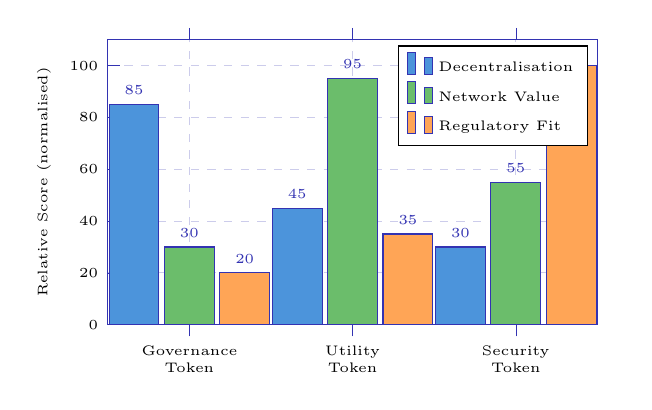
\begin{tikzpicture}
\begin{axis}[
  ybar,
  bar width=18pt,
  width=7.8cm,
  height=5.2cm,
  symbolic x coords={Governance,Utility,Security},
  xtick=data,
  xticklabels={Governance\\Token, Utility\\Token, Security\\Token},
  xticklabel style={font=\tiny, text width=2.5cm, align=center},
  ymin=0, ymax=110,
  ytick={0,20,40,60,80,100},
  yticklabel style={font=\tiny},
  ylabel style={font=\tiny},
  ylabel={Relative Score (normalised)},
  axis line style={draw=mlpurple},
  tick style={draw=mlpurple},
  nodes near coords,
  nodes near coords style={font=\tiny, color=mlpurple},
  point meta=y,
  enlarge x limits=0.25,
  grid=major,
  grid style={dashed, mllavender3},
  legend style={font=\tiny, at={(0.98,0.98)}, anchor=north east},
  legend cell align=left,
]
\addplot[fill=mlblue!70,  draw=mlpurple] coordinates {(Governance,85)(Utility,45)(Security,30)};
\addplot[fill=mlgreen!70, draw=mlpurple] coordinates {(Governance,30)(Utility,95)(Security,55)};
\addplot[fill=mlorange!70, draw=mlpurple] coordinates {(Governance,20)(Utility,35)(Security,100)};
\legend{Decentralisation, Network Value, Regulatory Fit}
\end{axis}
\end{tikzpicture}
\end{column}
\begin{column}{0.36\textwidth}
\vspace{4mm}
\begin{block}{Key Metrics}
\begin{itemize}\setlength\itemsep{4pt}
  \item[\small$\checkmark$] \small \textbf{\$2.5T+} total crypto market cap
  \item[\small$\checkmark$] \small \textbf{95\%} of new tokens fail within 3 years
  \item[\small$\checkmark$] \small \textbf{500+} bonding curve protocols deployed
  \item[\small$\checkmark$] \small \textbf{\$50B+} staked in governance tokens
  \item[\small$\checkmark$] \small \textbf{10x} spread between best/worst tokenomics
\end{itemize}
\end{block}
\end{column}
\end{columns}
\bottomnote{Tokenomics determines whether a protocol thrives or fails: governance tokens enable decentralisation, utility tokens power network activity, and security tokens bridge TradFi and DeFi.}
\end{frame}

% Frame 3: Token Economy Ecosystem
\begin{frame}{Token Economy Ecosystem}
\vspace{2mm}
\begin{center}
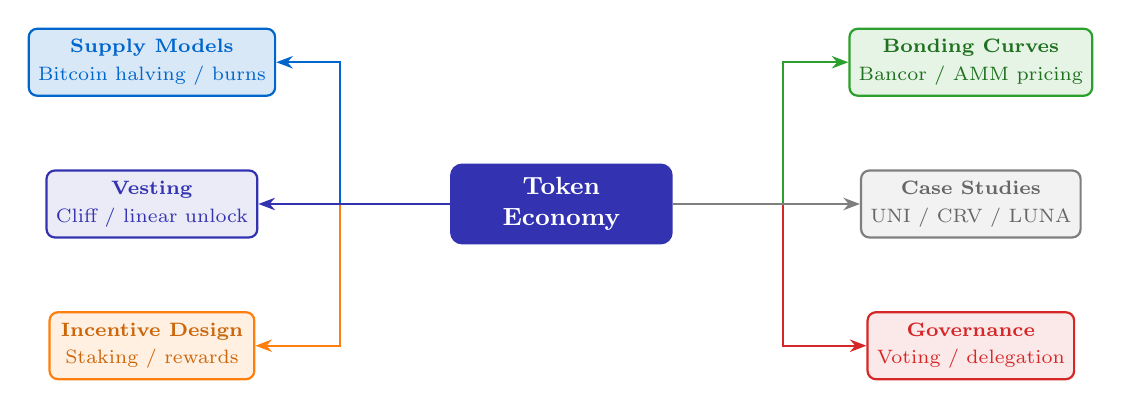
\begin{tikzpicture}[
  cbox/.style={rectangle, rounded corners=4pt, draw=mlpurple, thick,
               fill=mlpurple, minimum width=2.8cm, minimum height=1.0cm,
               font=\small\bfseries, align=center, text=white},
  sbox/.style={rectangle, rounded corners=3pt, thick,
               minimum width=2.6cm, minimum height=0.85cm,
               font=\scriptsize, align=center},
  arr/.style={-{Stealth[length=6pt]}, thick}
]
% Center node
\node[cbox] (center) at (0,0) {Token\\Economy};

% Spoke nodes
\node[sbox, draw=mlblue,   fill=mlblue!15,   text=mlblue]              (supply)  at (-5.2, 1.8)
  {\textbf{Supply Models}\\[2pt]Bitcoin halving / burns};

\node[sbox, draw=mlgreen,  fill=mlgreen!12,  text=mlgreen!70!black]    (bonding) at ( 5.2, 1.8)
  {\textbf{Bonding Curves}\\[2pt]Bancor / AMM pricing};

\node[sbox, draw=mlorange, fill=mlorange!12, text=mlorange!80!black]   (incent)  at (-5.2,-1.8)
  {\textbf{Incentive Design}\\[2pt]Staking / rewards};

\node[sbox, draw=mlred,    fill=mlred!10,    text=mlred]               (govern)  at ( 5.2,-1.8)
  {\textbf{Governance}\\[2pt]Voting / delegation};

\node[sbox, draw=mlpurple, fill=mlpurple!10, text=mlpurple]            (vesting) at (-5.2, 0.0)
  {\textbf{Vesting}\\[2pt]Cliff / linear unlock};

\node[sbox, draw=mlgray,   fill=mlgray!10,   text=mlgray!80!black]     (cases)   at ( 5.2, 0.0)
  {\textbf{Case Studies}\\[2pt]UNI / CRV / LUNA};

% Arrows
\draw[arr, draw=mlblue]   (center.west) -- ++(-1.4,0) |- (supply.east);
\draw[arr, draw=mlgreen]  (center.east) -- ++(1.4,0)  |- (bonding.west);
\draw[arr, draw=mlorange] (center.west) -- ++(-1.4,0) |- (incent.east);
\draw[arr, draw=mlred]    (center.east) -- ++(1.4,0)  |- (govern.west);
\draw[arr, draw=mlpurple] (center.west) -- ++(-1.4,0) |- (vesting.east);
\draw[arr, draw=mlgray]   (center.east) -- ++(1.4,0)  |- (cases.west);
\end{tikzpicture}
\end{center}
\bottomnote{A token economy integrates supply design, pricing mechanisms, incentive structures, governance systems, vesting schedules, and real-world case studies into a coherent whole.}
\end{frame}

% Frame 4: Token Design Space Growth
\begin{frame}{Token Design Space Growth}
\begin{columns}[T]
\begin{column}{0.62\textwidth}
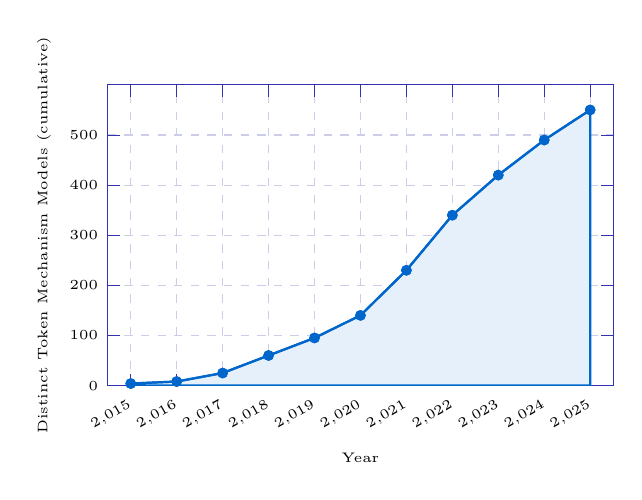
\begin{tikzpicture}
\begin{axis}[
  width=8.0cm,
  height=5.4cm,
  xmin=2014.5, xmax=2025.5,
  ymin=0, ymax=600,
  xtick={2015,2016,2017,2018,2019,2020,2021,2022,2023,2024,2025},
  ytick={0,100,200,300,400,500},
  xticklabel style={font=\tiny, rotate=30, anchor=north east},
  yticklabel style={font=\tiny},
  xlabel style={font=\tiny},
  ylabel style={font=\tiny},
  xlabel={Year},
  ylabel={Distinct Token Mechanism Models (cumulative)},
  axis line style={draw=mlpurple},
  tick style={draw=mlpurple},
  grid=major,
  grid style={dashed, mllavender3},
]
\addplot[color=mlblue, solid, thick, mark=*, mark size=1.5pt,
         fill=mlblue!10] coordinates {
  (2015,4)(2016,8)(2017,25)(2018,60)(2019,95)
  (2020,140)(2021,230)(2022,340)(2023,420)(2024,490)(2025,550)
} \closedcycle;
\addplot[color=mlblue, solid, thick, mark=*, mark size=1.5pt] coordinates {
  (2015,4)(2016,8)(2017,25)(2018,60)(2019,95)
  (2020,140)(2021,230)(2022,340)(2023,420)(2024,490)(2025,550)
};
\end{axis}
\end{tikzpicture}
\end{column}
\begin{column}{0.36\textwidth}
\vspace{4mm}
\begin{block}{Growth Drivers}
\begin{itemize}\setlength\itemsep{4pt}
  \item[\small$\checkmark$] \small \textbf{DeFi Summer} (2020) explosion of AMM/yield designs
  \item[\small$\checkmark$] \small \textbf{veTokenomics} (Curve) inspiring hundreds of forks
  \item[\small$\checkmark$] \small \textbf{NFT economies} adding novel royalty and burn mechanics
  \item[\small$\checkmark$] \small \textbf{L2 ecosystems} with bespoke sequencer token models
\end{itemize}
\end{block}
\end{column}
\end{columns}
\bottomnote{From 4 recognised token models in 2015 to over 550 by 2025, the design space has exploded --- making systematic tokenomics education more critical than ever.}
\end{frame}

% Frame 5: Course Coverage
\begin{frame}{Course Coverage}
\vspace{2mm}
\begin{center}
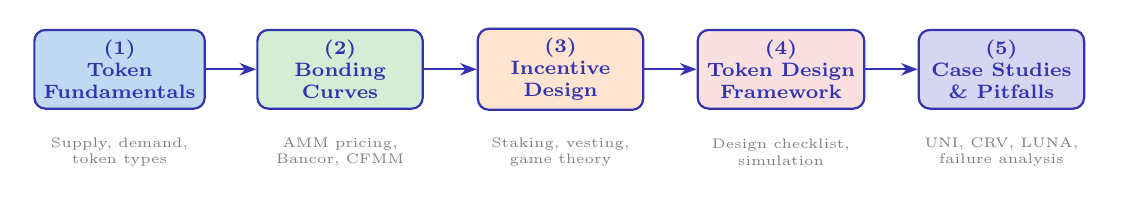
\begin{tikzpicture}[
  procstep/.style={
    rectangle, rounded corners=4pt,
    minimum width=2.1cm, minimum height=1.0cm,
    draw=mlpurple, thick,
    fill=mllavender3,
    font=\scriptsize\bfseries,
    align=center,
    text=mlpurple
  },
  conn/.style={-{Stealth[length=6pt]}, thick, draw=mlpurple}
]
\node[procstep, fill=mlblue!25]    (s1) at (0,0)    {(1)\\Token\\Fundamentals};
\node[procstep, fill=mlgreen!20]   (s2) at (2.8,0)  {(2)\\Bonding\\Curves};
\node[procstep, fill=mlorange!20]  (s3) at (5.6,0)  {(3)\\Incentive\\Design};
\node[procstep, fill=mlred!15]     (s4) at (8.4,0)  {(4)\\Token Design\\Framework};
\node[procstep, fill=mlpurple!20]  (s5) at (11.2,0) {(5)\\Case Studies\\\& Pitfalls};

\draw[conn] (s1) -- (s2);
\draw[conn] (s2) -- (s3);
\draw[conn] (s3) -- (s4);
\draw[conn] (s4) -- (s5);

\node[font=\tiny, text=mlgray, align=center, text width=2.1cm] at (0,-1.05)
  {Supply, demand,\\token types};
\node[font=\tiny, text=mlgray, align=center, text width=2.1cm] at (2.8,-1.05)
  {AMM pricing,\\Bancor, CFMM};
\node[font=\tiny, text=mlgray, align=center, text width=2.1cm] at (5.6,-1.05)
  {Staking, vesting,\\game theory};
\node[font=\tiny, text=mlgray, align=center, text width=2.1cm] at (8.4,-1.05)
  {Design checklist,\\simulation};
\node[font=\tiny, text=mlgray, align=center, text width=2.1cm] at (11.2,-1.05)
  {UNI, CRV, LUNA,\\failure analysis};
\end{tikzpicture}
\end{center}
\vspace{4mm}
\begin{columns}[T]
\begin{column}{0.48\textwidth}
\begin{block}{Prerequisites}
\begin{itemize}\setlength\itemsep{2pt}
  \item[\small$\checkmark$] \small Basic blockchain and DeFi concepts
  \item[\small$\checkmark$] \small Introductory microeconomics and game theory
\end{itemize}
\end{block}
\end{column}
\begin{column}{0.48\textwidth}
\begin{block}{Outcomes}
\begin{itemize}\setlength\itemsep{2pt}
  \item[\small$\checkmark$] \small Design and critically evaluate token economic systems
  \item[\small$\checkmark$] \small Identify failure modes and apply mechanism design principles
\end{itemize}
\end{block}
\end{column}
\end{columns}
\bottomnote{Five modules progress from foundational token economics through bonding curve mathematics, incentive engineering, and a structured design framework to real-world case studies.}
\end{frame}

% Frame 6: What You Will Learn
\begin{frame}{What You Will Learn}
\begin{columns}[T]
\begin{column}{0.44\textwidth}
\vspace{2mm}
\begin{block}{Learning Outcomes}
\begin{itemize}\setlength\itemsep{5pt}
  \item[\small$\checkmark$] \small \textbf{Supply models} --- analyse Bitcoin halving, token burns, and inflation schedules
  \item[\small$\checkmark$] \small \textbf{Bonding curves} --- derive AMM pricing, liquidity depth, and slippage
  \item[\small$\checkmark$] \small \textbf{Game theory} --- design incentive-compatible staking and reward systems
  \item[\small$\checkmark$] \small \textbf{Vesting \& governance} --- structure cliff schedules and voting power
  \item[\small$\checkmark$] \small \textbf{Real-world analysis} --- dissect UNI, CRV, and the LUNA collapse
\end{itemize}
\end{block}
\end{column}
\begin{column}{0.54\textwidth}
\vspace{2mm}
\begin{center}
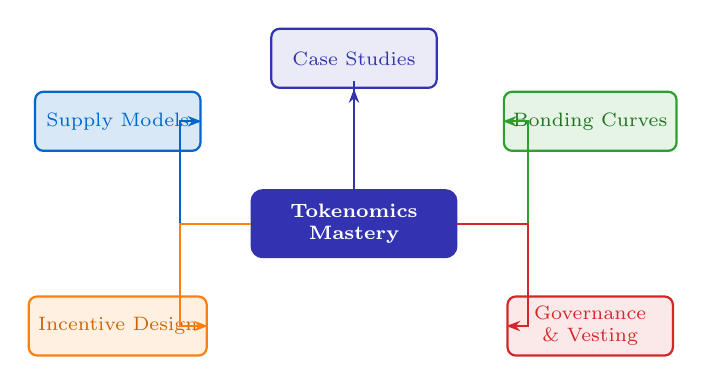
\begin{tikzpicture}[
  cbox/.style={rectangle, rounded corners=4pt, draw=mlpurple, thick,
               fill=mlpurple, minimum width=2.6cm, minimum height=0.85cm,
               font=\scriptsize\bfseries, align=center, text=white},
  fbox/.style={rectangle, rounded corners=3pt, thick,
               minimum width=2.1cm, minimum height=0.75cm,
               font=\scriptsize, align=center},
  farr/.style={-{Stealth[length=5pt]}, thick}
]
% Central node
\node[cbox] (nm) at (0,0) {Tokenomics\\Mastery};

% Skill nodes
\node[fbox, draw=mlblue,   fill=mlblue!15,   text=mlblue]              (sup)  at (-3.0, 1.3) {Supply Models};
\node[fbox, draw=mlgreen,  fill=mlgreen!12,  text=mlgreen!70!black]    (bon)  at ( 3.0, 1.3) {Bonding Curves};
\node[fbox, draw=mlorange, fill=mlorange!12, text=mlorange!80!black]   (inc)  at (-3.0,-1.3) {Incentive Design};
\node[fbox, draw=mlred,    fill=mlred!10,    text=mlred]               (gov)  at ( 3.0,-1.3) {Governance\\\& Vesting};
\node[fbox, draw=mlpurple, fill=mlpurple!10, text=mlpurple]            (cas)  at ( 0.0, 2.1) {Case Studies};

% Arrows
\draw[farr, draw=mlblue]   (nm.west)  -- ++(-0.9,0) |- (sup.east);
\draw[farr, draw=mlgreen]  (nm.east)  -- ++(0.9,0)  |- (bon.west);
\draw[farr, draw=mlorange] (nm.west)  -- ++(-0.9,0) |- (inc.east);
\draw[farr, draw=mlred]    (nm.east)  -- ++(0.9,0)  |- (gov.west);
\draw[farr, draw=mlpurple] (nm.north) -- ++(0,0.6)  |- (cas.south);
\end{tikzpicture}
\end{center}
\end{column}
\end{columns}
\vspace{1mm}
\bottomnote{By the end you will be able to design, simulate, and critically evaluate token economic systems using supply models, bonding curve mathematics, and mechanism design principles.}
\end{frame}

\end{document}
